\newpage
\section{Design patterns utilizzati}
Nella progettazione di MaaS sono stati utilizzati i seguenti design patterns:
\begin{itemize}
\item \textbf{Builder};
\item \textbf{Facade};
\item \textbf{Singleton};
\item \textbf{Chain of Responsability}.
\end{itemize}
Verrà presentata una descrizione questi design pattern, dividendoli in base al loro tipo, ovvero:
\begin{itemize}
\item \textbf{Creazionali}: Builder e Singleton.
\item \textbf{Strutturali}: Facade.
\item \textbf{Comportamentali}: Chain of responsability.
\end{itemize}
\subsection{Creazionali}
\subsubsection{Builder}
\paragraph{Descrizione} \mbox{} \\
Il design pattern Builder separa la costruzione di un oggetto complesso dalla sua rappresentazione cosicché il processo di costruzione stesso possa creare diverse rappresentazioni. L'algoritmo per la creazione di un oggetto complesso è indipendente dalle varie parti che costituiscono l'oggetto e da come vengono assemblate. \\
Ciò ha l'effetto immediato di rendere più semplice la classe, permettendo a una classe builder separata di focalizzarsi sulla corretta costruzione di un'istanza e lasciando che la classe originale si concentri sul funzionamento degli oggetti. Questo è particolarmente utile quando si vuole assicurare che un oggetto sia valido prima di istanziarlo, e non si vuole che la logica di controllo appaia nei costruttori degli oggetti. Un builder permette anche di costruire un oggetto passo-passo, cosa che si può verificare quando si fa il parsing di un testo o si ottengono i parametri da un'interfaccia interattiva. \\
A differenza dei design pattern Abstract Factory e Factory Method, il cui scopo è permettere il polimorfismo, l'intenzione del Builder è quella di ridurre il cosiddetto effetto telescoping nei costruttori, che porta ad un grande numero di parametri richiesti in fase di costruzione dell'oggetto.
\paragraph{Vantaggi} \mbox{} \\
\begin{itemize}
\item Permette di variare la rappresentazione interna di un oggetto.
\item Incapsula il codice della costruzione.
\item Fornisce maggiore controllo sui passi di costruzione dell'oggeto.
\end{itemize}
\paragraph{Svantaggi} \mbox{} \\
\begin{itemize}
\item Richiede la crezione di un oggetto separato (ConcreteBuilder) per ogni tipo di oggetto da costruire (Product).
\end{itemize}
\paragraph{Struttura}
\begin{figure}[h]
\centering
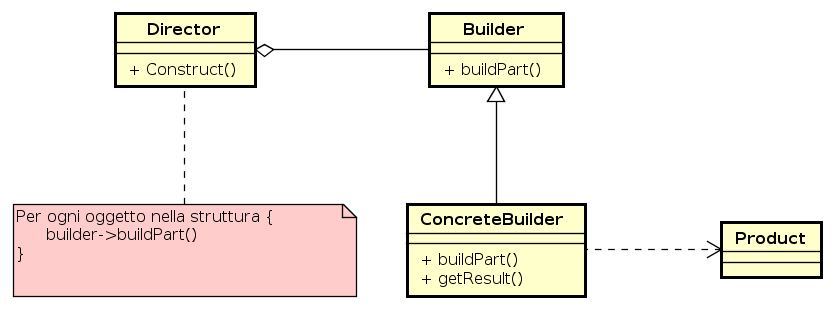
\includegraphics[width=0.8\textwidth]{res/sections/backend/builder.png}
\caption{Diagramma di deployment per l'architettura}
\end{figure}
\subsubsection{Singleton}
\paragraph{Descrizione} \mbox{} \\
Lo scopo del design pattern creazionale denominato Singleton è assicurare l’esistenza di un'unica istanza di una classe e fornire un punto di accesso globale ad essa. Questo pattern è nato per rispondere alla necessità di non avere più istanze della stessa classe, anche nei linguaggi in cui non è possibile usare una variabile globale, pur dando la possibilità alla classe di tener traccia di quella sua istanza. Il Singleton è quindi applicabile ogniqualvolta debba esistere una sola istanza di una certa classe in tutta l’applicazione, prestando però attenzione al fatto che l’istanza sia estendibile tramite ereditarietà.
\paragraph{Vantaggi} \mbox{} \\
\begin{itemize}
\item Controllo completo di come e quando i client accedono all’interfaccia della classe.
\item Evita l’utilizzo ingiustificato di variabili globali.
\item Consente di ridefinire le operazioni definite nel Singleton.
\item Permette di porre un limite massimo al numero di istanze di una certa classe.
\end{itemize}
\paragraph{Svantaggi} \mbox{} \\
\begin{itemize}
\item Può essere usato male e solo per modellare una variabile globale.
\item Viola il Single Responsability Principle: controlla sia la propria creazione che il proprio ciclo di vita.
\end{itemize}
\paragraph{Struttura} \mbox{} \\
\begin{figure}[h]
\centering
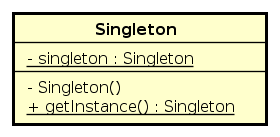
\includegraphics[width=0.8\textwidth]{res/sections/backend/singleton.png}
\caption{Diagramma di deployment per l'architettura}
\end{figure}
\subsection{Strutturali}
\subsubsection{Facade}
\paragraph{Descrizione} \mbox{} \\
Questo design pattern fornisce un'interfaccia unificata per un insieme di interfacce presenti in un sottosistema. Facade definisce un'interfaccia di alto livello che rende il sottosistema più semplice da utilizzare. Suddividere un sistema in sottosistemi aiuta a ridurne la complessità. Il suo scopo è rendere una libreria più facile da usare, capire, testare e leggere, riducendo al contempo le dipendenze da codice esterno per le operazioni interne. Di solito si usa quando:
\begin{itemize}
\item un'interfaccia semplice deve accedere ad un sistema complesso;
\item l'astrazione e l'implementazione sono molto accoppiate;
\item si necessita di un punto di entrata per ogni livello di un software a strati;
\item un sistema è molto complesso e difficile da capire.
\end{itemize}
\paragraph{Vantaggi} \mbox{} \\
\begin{itemize}
\item Disaccoppia il sottosistema dai client e dagli altri sottosistemi, promuovendo quindi la portabilità e l'indipendenza di sottosistemi.
\item Permette di organizzare i sottosistemi in una struttura a livelli.
\item Fornisce una vista semplice di base su un sottosistema che si rivela essere sufficiente per la maggior parte dei client.
\end{itemize}
\paragraph{Svantaggi} \mbox{} \\
\begin{itemize}
\item Non aggiunge funzionalità, semplifica solamente le interfacce.
\end{itemize}
\paragraph{Struttura} \mbox{} \\
\begin{figure}[h]
\centering
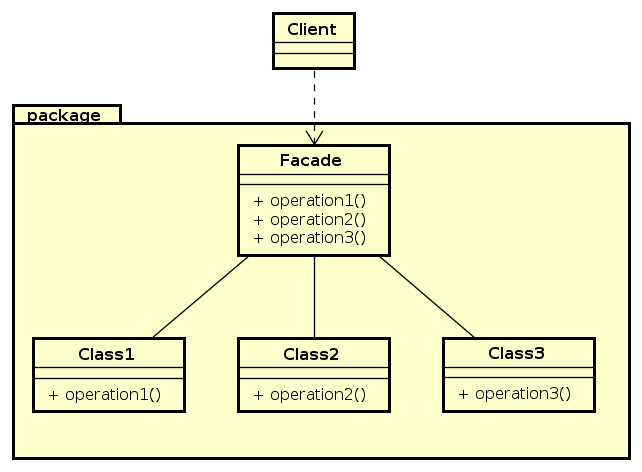
\includegraphics[width=0.8\textwidth]{res/sections/backend/facade.png}
\caption{Diagramma di deployment per l'architettura}
\end{figure}
\subsection{Comportamentali}
\subsubsection{Chain of responsability}
\paragraph{Descrizione} \mbox{} \\
Il Chain of Responsibility permette di separare i sender dai receiver delle richieste. La richiesta attraversa una catena di oggetti per essere intercettata solo quando raggiunge il proprio gestore. Viene utilizzato quando non è possibile determinare staticamente il receiver oppure l’insieme di oggetti gestori cambia dinamicamente a runtime. \\
Le richieste vengono dette implicite poiché il sender non ha alcuna conoscenza sull’identità del ricevente. Per permettere alla richiesta di attraversare la catena e per rimanere implicita, ogni receiver condivide un interfaccia comune per gestire le richieste ed accedere al proprio successore. La gerarchia che vorrà inviare richieste dovrà avere una superclasse che dichiara un metodo handler generico.
\paragraph{Vantaggi} \mbox{} \\
\begin{itemize}
\item Porta ad un accoppiamento debole tra i componenti.
\item Aggiunge flessibilità nell’assegnamento delle responsabilità degli oggetti.
\end{itemize}
\paragraph{Svantaggi} \mbox{} \\
\begin{itemize}
\item Non c’è garanzia che la request venga gestita: questo può avvenire quando la catena non è stata costruita in modo rigoroso.
\end{itemize}
\paragraph{Struttura} \mbox{} \\
\begin{figure}[h]
\centering
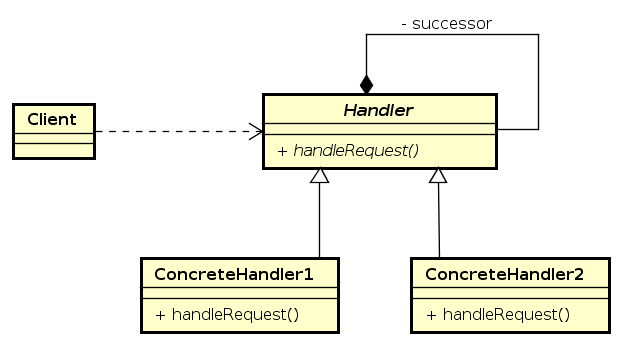
\includegraphics[width=0.8\textwidth]{res/sections/backend/chainOfResponsability.png}
\caption{Diagramma di deployment per l'architettura}
\end{figure}